% The hole cube with top T and generators X_1, X_2, X_3.
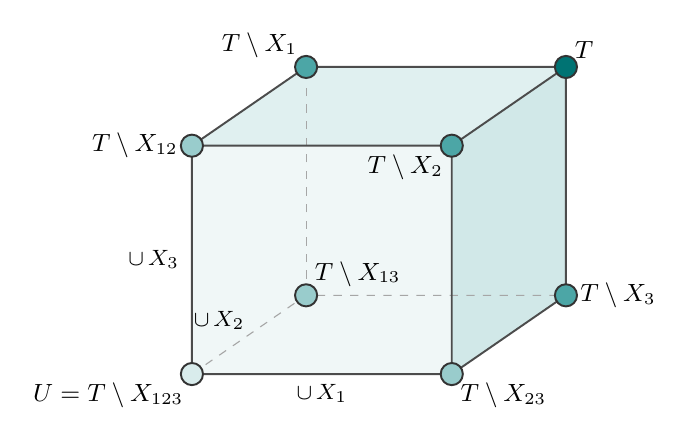
\begin{tikzpicture}[
    x={(3.3cm,0cm)}, y={(1.45cm,1.0cm)}, z={(0cm,2.9cm)},
    v/.style={circle, draw=black!80, line width=0.7pt, inner sep=0pt, minimum size=8pt},
    lab/.style={font=\small, inner sep=2pt},
    elab/.style={font=\footnotesize, inner sep=1.5pt, fill=white, fill opacity=0.85, text opacity=1}]
  \fill[teal!6]  (0,0,0) -- (1,0,0) -- (1,0,1) -- (0,0,1) -- cycle;
  \fill[teal!12] (0,0,1) -- (1,0,1) -- (1,1,1) -- (0,1,1) -- cycle;
  \fill[teal!18] (1,0,0) -- (1,1,0) -- (1,1,1) -- (1,0,1) -- cycle;
  \draw[dashed, gray!70] (0,0,0) -- (0,1,0) -- (1,1,0);
  \draw[dashed, gray!70] (0,1,0) -- (0,1,1);
  \draw[black!70, line width=0.7pt]
    (0,0,0) -- (1,0,0) -- (1,1,0) -- (1,1,1) -- (0,1,1) -- (0,0,1) -- cycle
    (1,0,0) -- (1,0,1) -- (1,1,1)
    (0,0,1) -- (1,0,1);
  % vertices, shaded by how many generators are removed
  \node[v, fill=teal!15] (U)   at (0,0,0) {};
  \node[v, fill=teal!40] (x1)  at (1,0,0) {};
  \node[v, fill=teal!40] (x2)  at (0,1,0) {};
  \node[v, fill=teal!40] (x3)  at (0,0,1) {};
  \node[v, fill=teal!70] (x12) at (1,1,0) {};
  \node[v, fill=teal!70] (x13) at (1,0,1) {};
  \node[v, fill=teal!70] (x23) at (0,1,1) {};
  \node[v, fill=teal!90!black] (T) at (1,1,1) {};
  \node[lab, below left=1pt]  at (U)   {$U=T\setminus X_{123}$};
  \node[lab, below right=1pt] at (x1)  {$T\setminus X_{23}$};
  \node[lab, above right=1pt] at (x2)  {$T\setminus X_{13}$};
  \node[lab, left=3pt]        at (x3)  {$T\setminus X_{12}$};
  \node[lab, right=3pt]       at (x12) {$T\setminus X_{3}$};
  \node[lab, below left=1pt]  at (x13) {$T\setminus X_{2}$};
  \node[lab, above left=1pt]  at (x23) {$T\setminus X_{1}$};
  \node[lab, above right=1pt] at (T)   {$T$};
  % what each edge direction does
  \node[elab, below=2pt] at (0.5,0,0) {$\cup\,X_1$};
  \node[elab, left=3pt]  at (0,0,0.5) {$\cup\,X_3$};
  \node[elab, fill=none, above left=0pt] at (0,0.5,0) {$\cup\,X_2$};
\end{tikzpicture}
